\documentclass[12pt]{article}


\usepackage[utf8]{inputenc}
\usepackage[T1]{fontenc}
\usepackage[francais]{babel}
\usepackage{listings}
\usepackage{color}
\usepackage{graphicx}
\usepackage{makeidx}
\usepackage{tikz}
\usepackage{caption}
\usepackage{float}
\usepackage{mathtools}
\usepackage[top=3cm, bottom=2cm, left=5cm, right=4cm]{geometry}



\lstset{
language = Java,
numbers=left,
numbersep=7pt,
backgroundcolor=\color{white},
frame=L,
showstringspaces=false,
mathescape = true;
}



\title{Spécifications techniques}
\author{Aurélien \bsc{Svevi}}
\date{14 mars 2015}
\begin{document}
\maketitle

\tableofcontents

\newpage
\addcontentsline{toc}{part}{Technologies employés}
\part*{Technologies employés}
\begin{itemize}
\item Nous coderons notre projet en langage java avec les normes de développement fournis.
\\
\item Pour le partage des donnés nous utiliserons le logiciel \textbf{git} qui nous permettra de conserver un historique de toutes les modifications sur le projet.


\end{itemize}

\newpage
\addcontentsline{toc}{part}{Fonctionnement du jeu}
\part*{Fonctionnement du jeu}
\section{Le plateau de jeu}
Le plateau de jeu sera composé d'un certaine nombre de \emph{Position} définit par l'utilisateur.
Pour ce faire nous disposerons d'une class \emph{map} contenant une hashmap de \emph{Position} avec comme clé un String contenant une lettre et un chiffre (c4,a2...) et comme valeur une instance de la case.
De plus chaque cases aura plusieurs attributs booleans permettant de savoir ce qui est présent sur cette case (base, obstacle, mine...)

\section{les robots}
Il y a 3 types de robots :Tireur, piégeur et char.
Tous ces robots ont des caractéristiques qui leurs sont propres (portée, vie, déplacement...) en revanche leur fonctionnement est semblable, ils peuvent tous se déplacer, attaquer et sont tous sur une \emph{cases}.

Ainsi nous allons créer une class abstraite \emph{Robot}. Dans cette class nous créerons divers fonctions visant à gérer la vie des robots, leur position...,
Ensuite nous créerons 3 autres class : \emph{Piegeur} , \emph{Tireur} et \emph{Char} qui hériterons de la class \emph{Robot} et dans laquelle nous ajouterons les éventuels particularité des robots (quantité de mines...).

\section{les attaques}
Pour gérer l'attaque des robots qui diffère de l'un à l'autre (par exemple, le piégeur pour attaquer pose une mine) nous allons créer une class \emph{attaque}.
Cette class aura 2 constructeurs:
\begin{itemize}
\item Un constructeur avec 2 robots en paramètres
\item Un constructeur avec 1 robot et une case en paramètre
\end{itemize}
Ainsi par exemple, le piégeur ciblera une case pour poser sa mine alors que le char ciblera un autre robot pour attaquer.

\newpage
\addcontentsline{toc}{part}{Algorithmes complexes}
\part*{Algorithmes complexes}
\setcounter{section}{0}

\section{Chemin disponible à travers les obstacles}
Sur la carte, seront disposés des obstacle mais avec une contrainte : toujours avoir un chemin possible entre la bas A et la base B.
\\
\begin{lstlisting}
List<case> chemin;
case c = new case();

Tant que c n'est pas sur la base oppose au depart:
	Se deplacer aleatoirement (x+1 || y+1)
	Mettre a jour c avec les nouvelles positions
	chemin.add(new case(c.x,c.y);

int nbrObstacles; //nbrObstacle ne doit pas 
		//depasser (largeur+hauteur)/2

Pour i allant de 1 a nbrObstacles:
	Tirer une case aleatoirement dans 
	la hashmap de la carte
	
	SI case appartient a chemin:
		case.obstacle = vrai
	SINON:
		Tirer une autre case
		
\end{lstlisting}
\newpage
\section{Déplacement des robots}
Les robots en fonction de leur type ne se déplacent pas de la même manière:
\begin{lstlisting}
position caseActuel = robot.pos
position caseCible

SI((robot instance of Tireur || robot instance of Piegeur) &&
 caseCible.x == caseActuel.x +/- 1 ||
 caseCible.y == caseActuel.y +/- 1):
	 
	robot.pos = caseCible

SINON SI:((robot instance of Char) && 
 caseCible.x == caseActuel.x +/- 2 XOR
 caseCible.y == caseActuel.y +/- 2):'
 
	robot.pos = caseCible
\end{lstlisting}

\section{Historique et sauvegarde}
Au cours de la partie, toutes les actions des joueurs seront stockés dans un tableau.
Ainsi, lorsque le joueur demande à sauvegarder sa partie, nous créerons un fichier texte sous cette forme:
\begin{lstlisting}
//en-tete
Nom de la sauvegarde
Nombre d'obstacles
Nombre de robots et type de chacun

//corps du fichier
robot realisant le deplacement -- type d'action -- case cible
4 1 c4
6 0 c1
\end{lstlisting}
Lors du chargement, La partie sera refaite entièrement jusqu'à arrivé à la fin du fichier ce qui permettra de revenir au moment de la sauvegarde.

\newpage
\section{Vérifier si au moins un robot est hors de la base}
Le joueur est toujours obligé d'avoir au moins un robot en dehors de sa base, sauf le premier tour ou alors si le joueur a perdu tous ses robots. Ainsi il faudra vérifier à chaque tour si au moins un robot est dehors grâce à cet algorithme:

\begin{lstlisting}
int nbrTotalRobots;
Robot[] tab;

POUR(i allant de 0 a nbrTotalRobots):

	SI(!tab[i].position.base):
		retourne vrai

retourne faux
\end{lstlisting}


\addcontentsline{toc}{part}{UML}
\part*{UML}

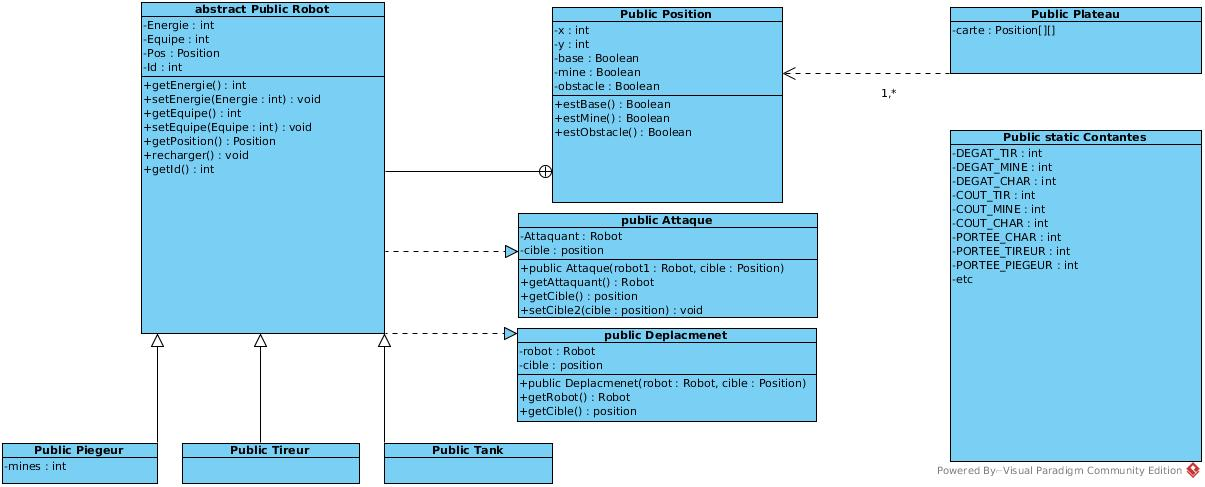
\includegraphics[scale=0.4, angle = -90]{img/uml.jpg}

\end{document}



